\section{Results}\label{sec-results}

\subsection{Quantitative analysis}\label{sub-sec-quantitativeanalysis}

Regarding the causes, the number of journalistic pieces registered on
traffic accidents stands out from the rest of the causes. There have
been 5,105 news items on traffic accidents out of the 5,727 total units
(which means 89.14\%). Drowning (8.03\%) is the second most considered
cause and accidental falls and suicides do not reach 2\% of the total
(see \Cref{tab-01}).

\begin{table}[!htpb]
\centering
\begin{threeparttable}
\caption{Number of news according to type of claim by each media (2010-2020).}
\label{tab-01}
\begin{tabular}{*{7}{l}}
\toprule
& Traffic & Drowning & Falls & Suicides & Totals & \% \\
\midrule
\url{20minutos.es} & 1,832 & 123 & 13 & 7 & 1,975 & 34.49 \\
\url{abc.es} & 1,558 & 154 & 10 & 36 & 1,758 & 30.70 \\
\url{lavanguardia.com} & 906 & 76 & 8 & 25 & 1,015 & 17.72 \\
\url{elmundo.es} & 499 & 65 & 5 & 26 & 595 & 10.39 \\
\url{elconfidencial.com} & 192 & 26 & 8 & 11 & 237 & 4.14 \\
\url{elpais.com} & 118 & 16 & 9 & 4 & 147 & 2.57 \\
Totals & 5,105 & 460 & 53 & 109 & 5,727 & \\
\% & 89.14 & 8.03 & 0.93 & 1.90 & & 100.00 \\
\bottomrule
\end{tabular}
\source{Own elaboration.}
\end{threeparttable}
\end{table}

According to the type of media, according to their digital immigrant or
digital native nature, 3,515 journalistic pieces have been registered
for the former (\url{abc.es}, \url{lavanguardia.com}, \url{elmundo.es} and
\url{elpais.com}) and 2,212 for the latter (\url{20minutos.es} and
\url{elconfidencial.com}). As four digital immigrant media and two
digital native media have been considered, these data represent an
average of 1,106 news items published by each digital immigrant media
outlet and 879 news items by each digital native media outlet, which
indicates a 25.82\% greater coverage in news about accident events in
digital native media.

In the temporal analysis of the causes, a greater presence of traffic
accidents is observed than the rest and an increasing presence of this
type of accidents is confirmed in the media during the study period (see
\Cref{fig-01}).

\begin{figure}[htpb]
\centering
\begin{minipage}{\textwidth}
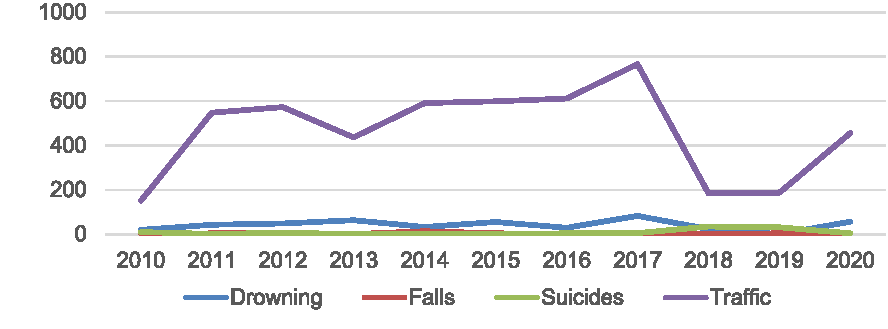
\includegraphics[width=\textwidth]{image1.pdf}
\caption{Evolution of the number of news items published by type of claim (2010-2020). Source: Own elaboration.}
\label{fig-01}
\source{Own elaboration.}
\end{minipage}
\end{figure}

If traffic accident events are published massively, it seems reasonable
to study whether this behavior responds to automated journalism where a
simple dump of information obtained by emergency services or information
agencies is performed. To study this effect, all identical headlines
published in different media have been selected, obtaining results that
reveal a high rate of exact coincidences (27.15\% of the news published
on traffic accidents) and media that produce this type of news very
little, as is the case of \emph{lavanguardia.com} with 66.23\% of the
news being exact to that of other media. In all the cases observed,
there is not only an exact match with the headline, but also with the
entire body of the message (see \Cref{tab-02}).

\begin{table}[!htpb]
\centering
\begin{threeparttable}
\caption{Number of identical traffic news for each media (2010-2020).}
\label{tab-02}
\begin{tabular}{*{4}{l}}
\toprule
 & Traffic news & Identical news & \% \\
\midrule
\url{20minutos.es} & 1,832 & 558 & 30.46 \\
\url{abc.es} & 1,558 & 96 & 6.16 \\
\url{lavanguardia.com} & 906 & 600 & 66.23 \\
\url{elmundo.es} & 499 & 53 & 10.62 \\
\url{elconfidencial.com} & 192 & 65 & 33.85 \\
\url{elpais.com} & 118 & 14 & 11.86 \\
Totals & 5,105 & 1,386 & 27.15 \\
\bottomrule
\end{tabular}
\source{Own elaboration.}
\end{threeparttable}
\end{table}

In total, 663 duplicated, 17 tripled and 6 quadrupled news items have
been detected, that is, the same headline and body of the news item is
repeated in exactly four media outlets at the same time.

To compare this effect with other causes, a coincidence analysis has
also been carried out between drowning news, which is the cause with the
second highest number of publications, where a high rate of accurate
news is also appreciated (see \Cref{tab-03}).

\begin{table}[!htpb]
\centering
\begin{threeparttable}
\caption{Number of identical drowning news for each media (2010-2020).}
\label{tab-03}
\begin{tabular}{*{4}{l}}
\toprule
& Drowning news & Identical news &\% \\
\midrule
\url{20minutos.es} & 123 & 43 & 34.96 \\
\url{abc.es} & 154 & 17 & 11.04 \\
\url{lavanguardia.com} & 76 & 48 & 63.16 \\
\url{elmundo.es} & 65 & 6 & 9.23 \\
\url{elconfidencial.com} & 26 & 15 & 57.69 \\
\url{elpais.com} & 16 & 1 & 6.25 \\
Totals & 460 & 130 & 28.26 \\
\bottomrule
\end{tabular}
\source{Own elaboration.}
\end{threeparttable}
\end{table}

In the case of news about accidental falls, the general coincidence
rates are maintained (it is even the highest rate recorded) and the
media that present identical news (\url{20minutos.es}, \url{lavanguardia.com}
and \url{elconfidencial.com}) are those that have been observed in the
previous analyzes that usually publish exact news in cases such as
traffic accidents and drowning (see \Cref{tab-04}).

\begin{table}[!htpb]
\centering
\begin{threeparttable}
\caption{Number of identical falls news for each media (2010-2020).}
\label{tab-04}
\begin{tabular}{*{4}{l}}
\toprule
& Falls news & Identical news &\%\\
\midrule
\url{20minutos.es} & 13 & 3 & 23.08 \\
\url{abc.es} & 10 & 0 & 0.00 \\
\url{lavanguardia.com} & 8 & 3 & 37.50 \\
\url{elmundo.es} & 5 & 0 & 0.00 \\
\url{elconfidencial.com} & 8 & 2 & 29.69 \\
\url{elpais.com} & 9 & 0 & 0.00 \\
Totals & 53 & 8 & 15.09 \\
\bottomrule
\end{tabular}
\end{threeparttable}
\end{table}

Finally, the same analysis has been carried out for the news about
suicides, where the coincidence rate drops significantly compared to
previous cases. In this case, the low number of news items published
(109) may reduce the representativeness of this analysis compared to
that carried out in the case of traffic accidents, where a greater
number of items is observed (5,727) (see \Cref{tab-05}).

\begin{table}[!htpb]
\centering
\begin{threeparttable}
\caption{Number of identical suicide news for each media (2010-2020).}
\label{tab-05}
\begin{tabular}{*{4}{l}}
\toprule
	& Suicide news & Identical news & \%\\
\midrule
\url{20minutos.es} & 7 & 0 & 0.00 \\
\url{abc.es} & 36 & 3 & 8.33 \\
\url{lavanguardia.com} & 25 & 4 & 16.00 \\
\url{elmundo.es} & 26 & 4 & 15.38 \\
\url{elconfidencial.com} & 11 & 1 & 9.09 \\
\url{elpais.com} & 4 & 0 & 0.00 \\
Totals & 109 & 12 & 11.00 \\
\bottomrule
\end{tabular}
\end{threeparttable}
\end{table}

\subsection{Qualitative analysis}\label{sub-sec-qualitativeanalysis}
\subsubsection{In-depth interviews}\label{sub-sub-sec-in-depthinterviews}

The media assume the use of official sources of information such as the
police, firefighters, courts, or authorities, but they also indicate
that they have their own sources that they seek over time.

\enquote{The main sources are the official ones: police forces, firefighters,
courts, authorities\ldots In some cases, it is also necessary to have
our own sources, apart from the official ones that provide additional
information. They are usually people who belong to any of the fields
mentioned above} (Jesús Morales, \emph{Diario de Noticias}).

\enquote{The elaboration is complex and seeks to draw on official sources and
the sources that have developed over the years in emergencies and police
forces} (Gabriel González, \emph{Diario de Navarra}).

Digital newspapers also acknowledge using official and unofficial
sources of information to write a news story, since it is essential for
them to compare the news with all those witnesses who may have
participated in the attention or observation of the event on which it is
reported.

\enquote{\ldots with the confirmation of the information by various sources or a
verified official source, it is important to have some important
aspects. Informatively, a source today can be anyone with direct access
to the event, but that alone is not enough when it comes to a relevant
event in which several people are involved, injured or dead. It is
essential to compare what happened with the security forces,
firefighters, heads of medical services or any other person who has been
able to participate professionally in dealing with the event} (Ignacio
Murillo, \url{Navarra.com}).

Journalists\textquotesingle associative organizations point out that
official sources of information should be considered a priority for
producing news on events.

\enquote{Generally, journalists always draw from official sources, such as the
police, citizen protection, and emergency services such as DYA (stop and
help) or the Red Cross\ldots These would be their first sources of access.
As they carry out the press release, they incorporate the information
from the journalist himself. The first information is what the
journalist receives when he arrives at the scene of the accident, and he
is the witness of what is happening. Then you must look for other
sources, which will be secondary sources of information, among which
there may be official sources} (Patxi Pérez, president of the
Association of Journalists of Navarre).

According to journalists, crimes and traffic accidents arouse more
interest in the audience. Regarding suicides, they believe that
information is offered in a very generic way and they even believe that
they are not discussed unless they have a public significance. They also
interpret that events related to accidental falls and suicides are
usually considered to be related to the private sphere and therefore are
not considered news material.

\enquote{Crimes are the content that arouses the most interest, followed by
accidents of all kinds: mountain, traffic, work, drowning\ldots Suicides
are news that are avoided unless they have a public significance,
although their treatment is always very limited} (Jesús Morales,
\emph{Diario de Noticias}).

\enquote{Of the accidental causes that you mention, only traffic accidents
report specific cases, while other causes, which belong more to the
private sphere, such as accidental falls and suicides, report more
global figures per year or through reports. About drowning, there are
few in Navarra and we never found out about many because, given the
suspicion that it could be a suicide, the sources do not even report
it} (Gabriel González, \emph{Diario de Navarra}).

From the point of view of the digital press, there is agreement in
pointing out that it is necessary to be demanding in the identification
of the victims and in the approach of the news. Ethics is part of the
training that the journalist receives, but his own experience should
allow him to know these limits.

\enquote{Reporting an event means always being much more demanding in all
aspects of the news, the identification of people or the approach of the
news (\ldots). All licensed or graduated journalists have received training
of this type, but it is when we get to real life that we must ask
ourselves where the limits are} (Ignacio Murillo, \url{Navarra.com}).

\subsubsection{Discussion group}\label{sub-sub-sec-discussiongroup}

According to the pre-established script, the moderator indicated that
the discussion would be divided into four different parts where topics
and questions would be raised for the participants to comment on and
interact with each other in order, brevity, and respect.

Beginning with the first part, the moderator indicated that the
objective in this block was to find out about society\textquotesingle s
perception of accidents and more specifically about suicides, accidental
falls, drowning and traffic accidents.

The participants of the discussion group perceived that this greater
social awareness about traffic accidents may be because this type of
news is the one that is published in greater numbers and that there is
additional institutional awareness (in this case a possible liability is
suggested policy when appointing the DGT) that promotes specific
prevention campaigns on this cause of accident. Therefore, it can be
appreciated that there may be deficiencies in the information offered by
the press on other types of claims.

\enquote{In other words, in the end, also within the subject of accidents, the
press should report a lot more, because one of the best ways to prevent
them in the future is to say how to avoid them [\ldots] Really the best
way to avoid these cases It would be saying from campaigns such as those
carried out by the DGT \enquote{zero tolerance with alcohol} or with drugs \enquote{if
you consume certain things, do not take the wheel} because it is not
only that you can end your life, if you cannot lead to the death of
other people} (M18).

When receiving this type of news, the members of the discussion group
indicate that society does not react and is generally conformist,
although a greater social response is perceived in the face of impactful
news regarding traffic accidents. Specifically, reference is made to an
accident that occurred on the N-121-A highway four days before the
meeting of this discussion group, where two people aged 21 and 19 died.
Forty-nine days after the event, \emph{Diario de Navarra} offers a piece
of news in its printed edition that occupies a third of the front page
in color, indicating: \enquote{One-hour demand cut on the N-121-A}. The
subtitle reads: \enquote{Some 1,500 residents demonstrate to demand that the
regional government give priority to security over economic cost.} In
central pages they report that \enquote{The future N-121-A will run in 2+2
between the Ezkaba and Oricáin roundabout and in 1+1 through the
Sorauren variant} (\emph{Diario de Navarra}, February 29, 2020).

\enquote{I think that doing little\ldots society little. But yes, for example
now there has been another\ldots two deaths in a traffic accident on
the Nacional 121, so I think that it does\ldots mobilize at least the
users of that road\ldots} (M58).

(Specificates) \enquote{The environment} (M68).

\enquote{[\ldots] those who use it more daily, those who use it more than I
don\textquotesingle t know what\ldots In the end it is the one that
promotes it, because of course, everyone knows that it is possibly the
most dangerous route here\ldots so always\ldots so that? How is it
fixed? Well, with money\ldots Instead of turning the road in the opposite
direction, you build a highway, and the death toll will be reduced\ldots
but\ldots I think that society must be aware of that} (M58).

Regarding the professionalism of the media, it is indicated that most
cases of news about events are limited to transcribing the press release
they receive from the emergency services or the police. This makes it
possible to locate the same news with an identical presentation in
different media.

\enquote{Two questions\ldots If we go to the treatment of the media, I believe
that basically the media do not do journalism, they do\ldots it is to dump
the press release of what the Provincial Police, the Civil Guard have
told them\ldots They don\textquotesingle t do more than that. And you look
at the news from \emph{Diario de Navarra} or \emph{Diario de Noticias}
and it\textquotesingle s the same} (M58).

The group proposes that the media carry out rigorous investigative work
to offer more complete information. The participants also indicate that
there must be prior social pressure for the government to act with
preventive measures.

\enquote{But you (referring to M58) have just said that, for example, the
information notes that are passed on to the newspapers is, well, through
the police\ldots the police that are passed on to the media\ldots So
maybe the media Communication simply transcribes what the police have
told you, but they don\textquotesingle t bother to investigate further.
So, ideally, that media outlet would be upset, right? In investigating
and giving the information I say, eh? I don\textquotesingle t know,
maybe I\textquotesingle m wrong} (F57).

\enquote{I think that with a topic it becomes social, the politician bends his
ears and starts working. If society does not get involved, in a more
majority way, or they do not feel that there is a pressure, they prefer
not to move\ldots That is clear} (F58).

\enquote{If you don\textquotesingle t exhaust them, even less}(M68).

The group is convinced to demand from the media information of social
interest about the accidents, with real data, rigorous reports, and
updated statistics, although they indicate that it is society itself
that is demanding much more information about other entertainment
content.

\enquote{And I think that just as we are the ones who must demand the
information we want. [\ldots] What\textquotesingle s happening? That if
it is not interesting, for us, for example, and for society, for a part
of society, these issues are interesting, (\ldots) that we have to move\ldots}
(F18).

\enquote{Why are three times as many banal information magazines sold, for
example, to the serious written press? Society is failing miserably.
Noisily} (M68).
